\subsubsection{Test \ref{test10}, \enquote{Is Connected?} button returns correct values for an acyclic graph, which \emph{is} connected.}
Input:  5 Vertices created, A, B, C, D, E.  Edge lines exist between (A, B), (A, C), (A, D), and (D, E). Click on the \enquote{Is Connected} button, observe the message in the status bar.
\newline
\newline
Expected output: The status bar should display \enquote{The graph is connected.}
\begin{figure}[ht]
    \centering
    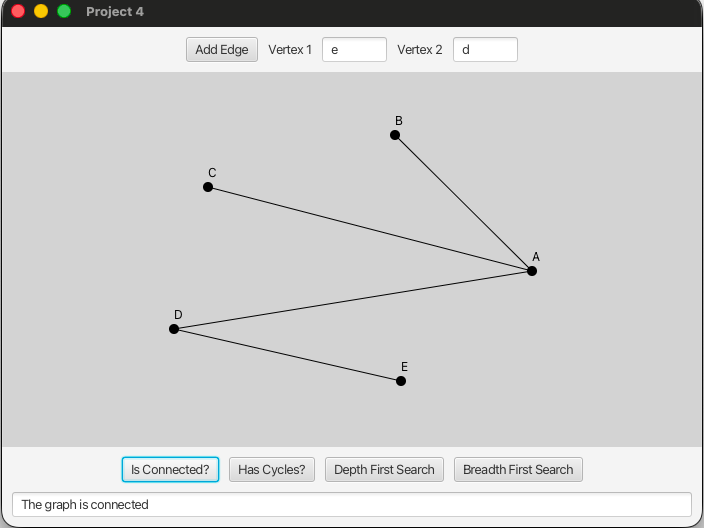
\includegraphics[width=0.65\textwidth]{images/test10.png}
    \caption{test \ref{test10}}
\end{figure}
